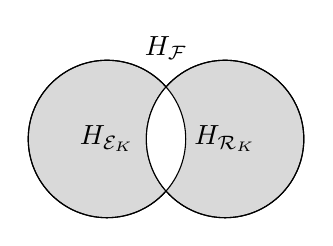
\begin{tikzpicture}
            % First circle
            \node[circle, draw, fill=gray!30, minimum size=2cm, label=center:\( H_{\mathcal{E}_K} \)] (HEK) at (0,0) {};

            % Second circle
            \node[circle, draw, fill=gray!30, minimum size=2cm, label=center:\( H_{\mathcal{R}_K} \)] (HRK) at (1.5,0) {};

            % Overlap drawing with white intersection
            \begin{scope}
                \clip (0,0) circle (1cm);
                \fill[white] (1.5,0) circle (1cm);
            \end{scope}

            % Redraw the circle borders to ensure they are visible
            \draw (0,0) circle (1cm);
            \draw (1.5,0) circle (1cm);

            % Label for the gray area moved above the intersection
            \node at (0.75,1.15) {\( H_{\mathcal{F}} \)};
        \end{tikzpicture}
